\subsection{Initializing}
After the user starts an application, an initialization step should happen to introduce itself to the other applications. This step uses the Device Introduction message. Figure \ref{fig:Initializing} shows a source application that joins the network and introduces itself with a message to library. Library publishes this message to all supported topics of Application State Models (e.g search), and the middleware forwards it to the library of the target application which subscribed to the same topic. Thereby, the library of the target application add the new device to a device list and notifies the target application about a new device. In response, target application introduce itself in the same way to the source application by using the before mentioned device specific subtopic for this specific application (e.g search/<source-device-uuid>).


\FloatBarrier \begin{figure}[H]
    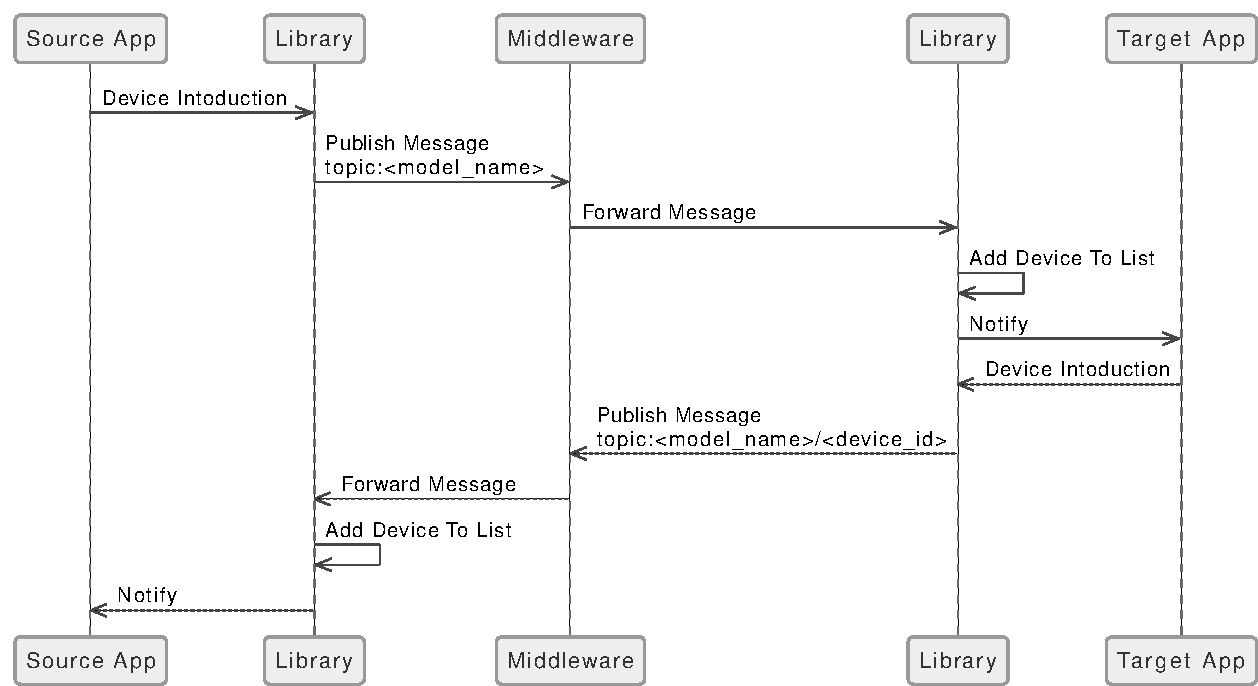
\includegraphics[width=\linewidth]{../figures/Initializing.pdf}
    \centering
    \caption{Initializing the Source Application}
    \label{fig:Initializing}
\end{figure} \FloatBarrier

\subsection{Going Offline}
An application might go offline intentionally or unintentionally, e.g. due to faults or network outages. A plan should cover these incidents. This step uses the Device Leave message. After disconnection, other devices are not allowed to send any message to that particular device.

\subsubsection{Graceful}
A user might close the application. In this case, the application goes offline gracefully, and it should notify other applications about its absence. Figure \ref{fig:Going-Offline-Graceful-Source} shows the source application going offline gracefully. With the library's help, the source application informs its absence to the middleware on \lstinline[basicstyle=\ttfamily]{online} topic, and the middleware forwards it to the library of the target application. Thereby, the library of the target application removes the device from devices list and notifies the target application about the leaving of the source application. 

\FloatBarrier \begin{figure}[H]
    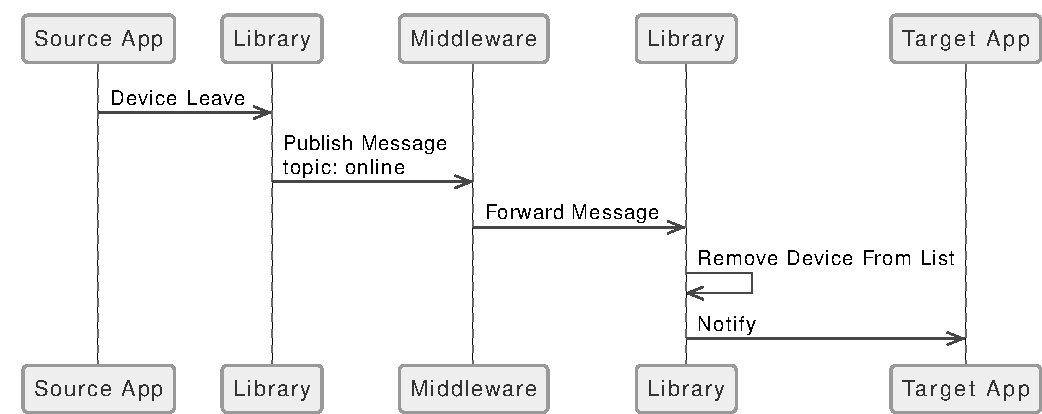
\includegraphics[width=\linewidth]{../figures/Going-Offline-Graceful-Source.pdf}
    \centering
    \caption{Going Offline Gracefully: Source}
    \label{fig:Going-Offline-Graceful-Source}
\end{figure} \FloatBarrier

\subsubsection{Ungraceful}
An application might go offline by other causes like network problems, device crashing, application failure, etc. In this case, the application goes offline ungracefully, and the middleware should notify other applications about its absence. Figure \ref{fig:Going-Offline-Ungraceful-Source} shows the source application going offline ungracefully. The middleware checks if the application is connected; if it does not get any response, request gets a timeout and it publishes a message to  \lstinline[basicstyle=\ttfamily]{online} topic. Thereby, the library of the target application removes the device from devices list notifies the target application about the leaving of the source application.

\FloatBarrier \begin{figure}[H]
    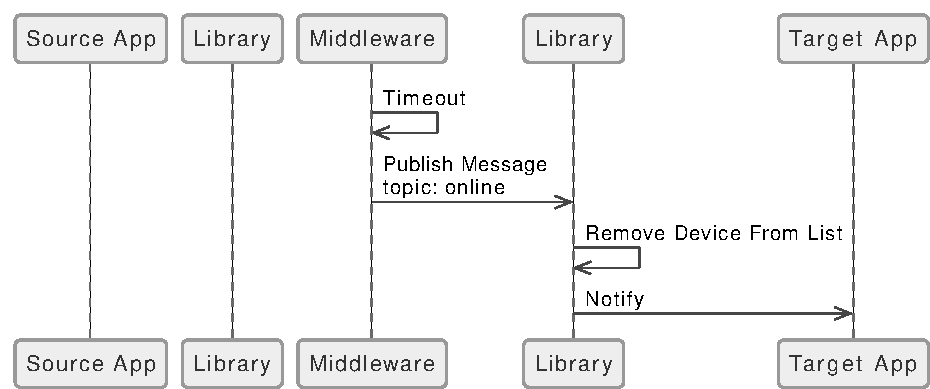
\includegraphics[width=\linewidth]{../figures/Going-Offline-Ungraceful-Source.pdf}
    \centering
    \caption{Going Offline Ungracefully: Source}
    \label{fig:Going-Offline-Ungraceful-Source}
\end{figure} \FloatBarrier

\subsubsection{Has Run-Time State}
Any application with a run-time state should notify other applications about having a run-time state, so that they aware that the run-time state exists and can be migrated. This step uses the Device Has State message. Figure \ref{fig:Inform-Devices-Has-State-Source} shows the source application has a run-time state and informs the middleware by publishing a message to topics of Application State Models and the middleware forward it to the library of the target application. Thereby, the library notifies the target application about the source application, which has a run-time state. The target application may react by enabling a button that would allow pulling the run-time state from the source to the target application. We explain these reactions later in Migration Patterns section.

\FloatBarrier \begin{figure}[H]
    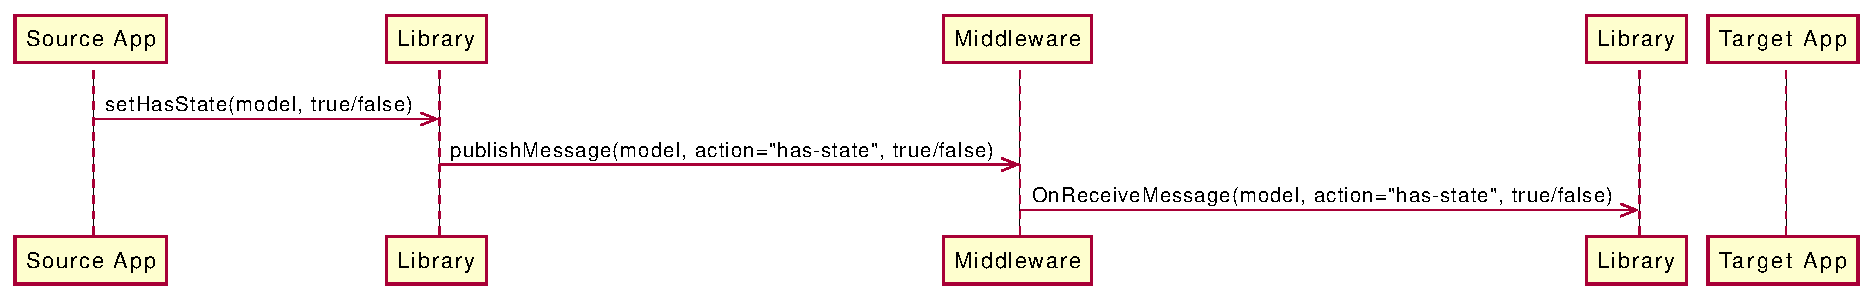
\includegraphics[width=\linewidth]{../figures/Inform-Devices-Has-State-Source.pdf}
    \centering
    \caption{Source App inform other devices that has a state}
    \label{fig:Inform-Devices-Has-State-Source}
\end{figure} \FloatBarrier

\subsection{Store Run-time State}
As different applications have different events for observing the changes on their current state information, run-time state should be temporarily stored and ready for migration if other applications request it. Figures \ref{fig:Store-Current-State-Source} shows that the source application can temporarily store its run-time state in the library.

\FloatBarrier \begin{figure}[H]
    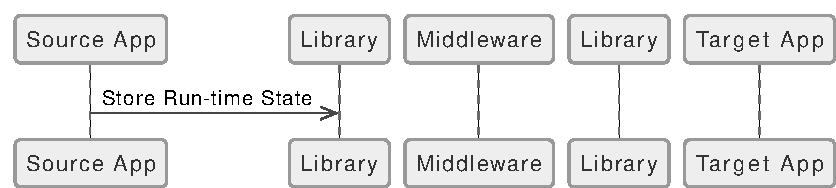
\includegraphics[width=\linewidth]{../figures/Store-Current-State-Source.pdf}
    \centering
    \caption{Source Application stores a run-time state in library.}
    \label{fig:Store-Current-State-Source}
\end{figure} \FloatBarrier


\subsection{Migration Patterns}
In this section, we describe two patterns for run-time state migration.

\subsubsection{Pull Method}
In the pull method, the target application request a run-time state from the source application. Figure \ref{fig:Pull-Method} shows the target application gets the list of devices with a common Application State Model, then selects the source application and requests its run-time state by sending a message from the library to the middleware. The middleware forwards the message, and the source application gets a request for migrating its run-time state. After processing the request, the source application sends its run-time state by the library to the middleware. The middleware forwards the message, and the target application receives the run-time state. The target application adjusts the new run-time state and remove its run-time state and notifies the source application about finalizing the run-time state migration by sending a message throw the library and the middleware. 

\FloatBarrier \begin{figure}[H]
    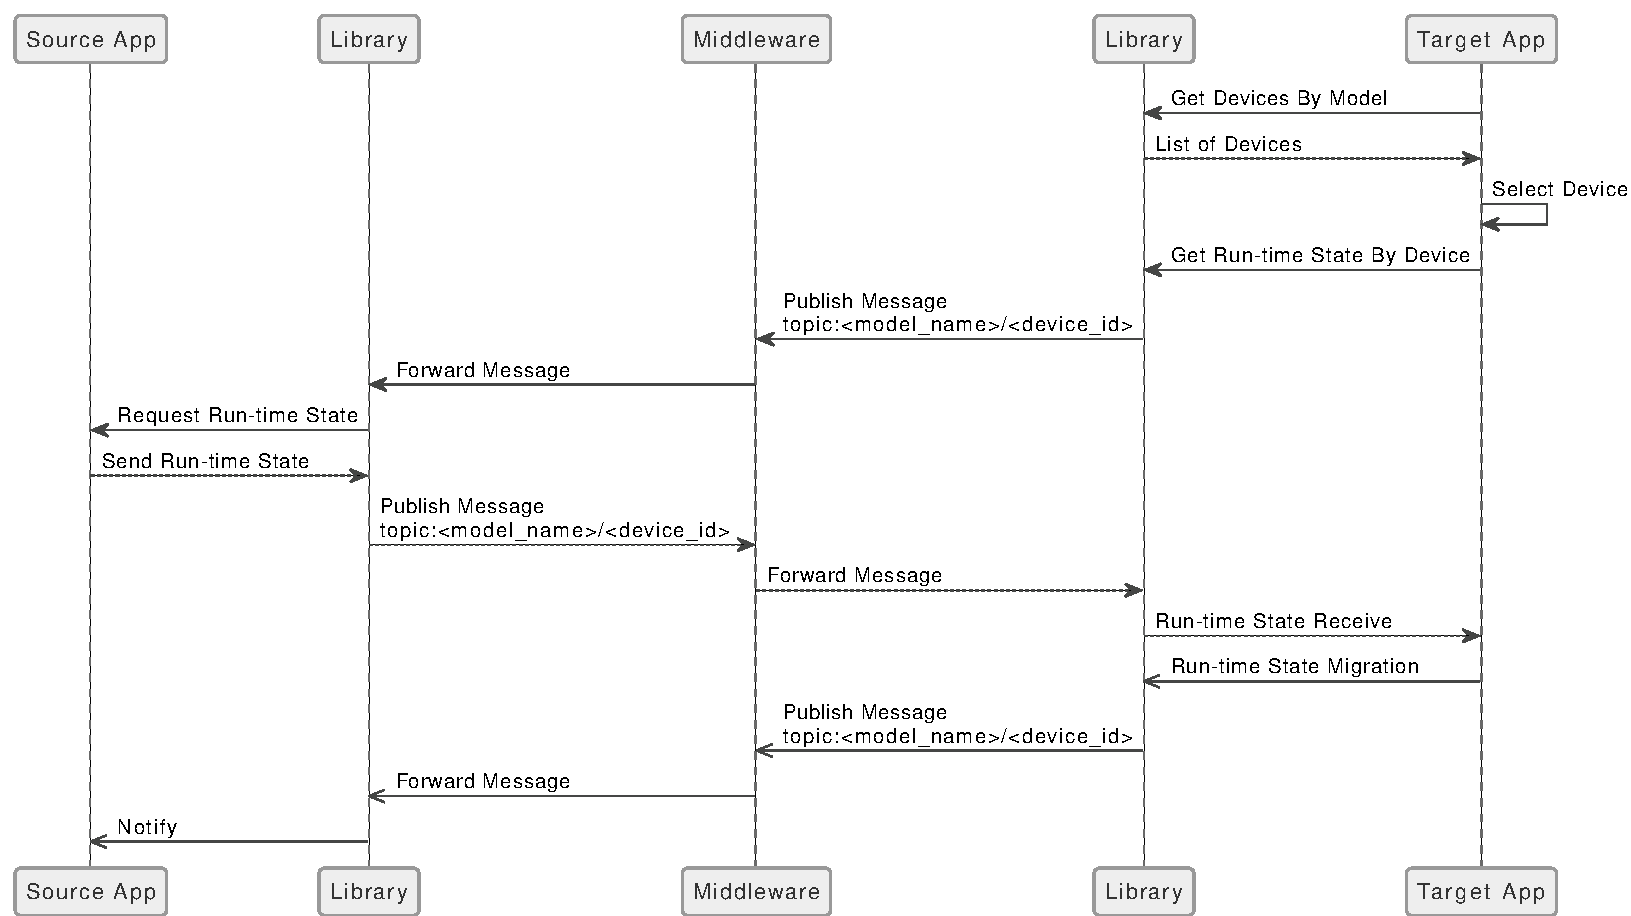
\includegraphics[width=\linewidth]{../figures/Pull-Method.pdf}
    \centering
    \caption{Pull Method: Migration Source to Target}
    \label{fig:Pull-Method}
\end{figure} \FloatBarrier

\subsubsection{Push Method}
In the push method, the source application send its run-time state to the target application without a request by force. Figure \ref{fig:Push-Method} shows the source application gets the list of devices with a common Application State Model, then selects the target application and requests its run-time state by sending a message from the library to the middleware. The middleware forwards the message, and the target application receives the run-time state. Target application adjusts the new run-time state and remove its run-time state and notifies the source application about finalizing the run-time state migration by sending a message throw the library and the middleware.

\FloatBarrier \begin{figure}[H]
    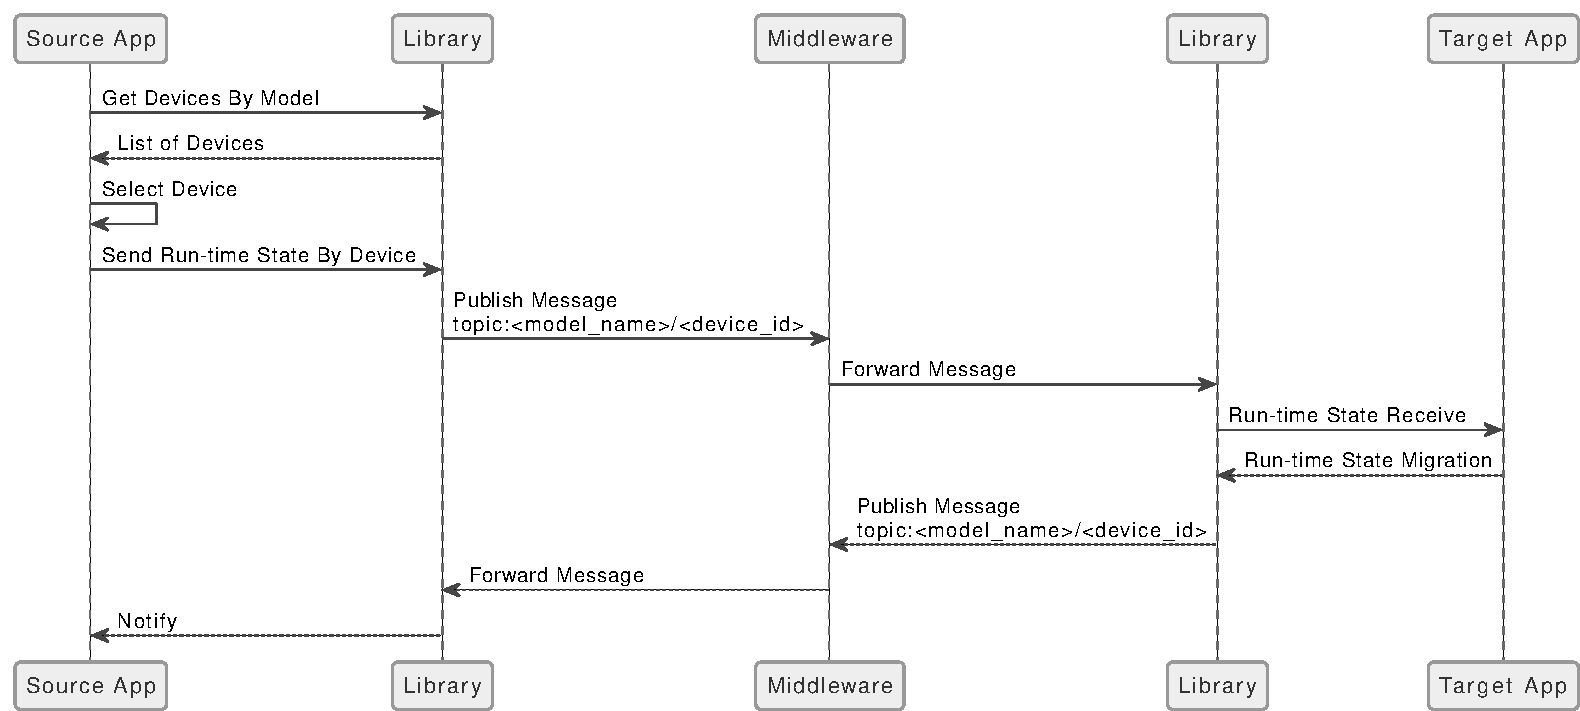
\includegraphics[width=\linewidth]{../figures/Push-Method.pdf}
    \centering
    \caption{Push Method: Migration Source to Target}
    \label{fig:Push-Method}
\end{figure} \FloatBarrier

